\subsection{Robot definition} 
En robot er en mekanisk enhed, der kan udføre opgaver enten automatisk eller med en hvis grad af menneskelig kontrol. Robotter spænder fra simple systemer med forudprogrammerede bevægelser til avancerede maskiner, der benytter sensorer og kunstig intelligens for at tilpasse sig skiftende omgivelser. De er en uundværlig del af moderne industri og forskning, hvor de bidrager til at øge præcision, effektivitet og ensartethed i arbejdsprocesser, der ellers ville kræve hårdt manuelt arbejde. 

I dette projekt handler det om at bruge robotteknologi til at automatisere påføringen af speckle patterns. Ved manuel påføring kan der opstå variationer, som påvirker målenøjagtigheden og gør det vanskeligt at reproducere resultater. En robot kan i stedet sikre en ensartet og præcis påføring, så mønstrene lever op til kravene for kontrast, fordeling og holdbarhed. For at kunne opnå dette skal robotten være i stand til at positionere sig korrekt, påføre mønstrene jævnt og tilpasse sig forskellige materialer og overflader.

\begin{figure} [H]
    \centering
    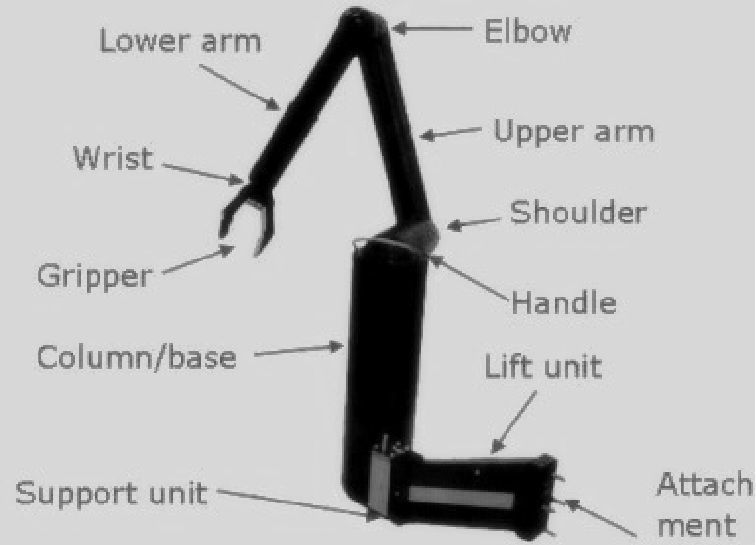
\includegraphics[width=0.7\linewidth]{Sections/2 Problemanalyse/Media/A-robotic-arm-with-labels-1.png}
    \caption{Robotarm med det vigtigste elementer angivet \parencite{ResearchGateALabels}}
    \label{fig:robotarm-navn}
\end{figure}

For at en robot kan udføre en opgave som denne, kræver det en række nøglekomponenter, der arbejder sammen. Robottens opbygning består af flere mekaniske elementer, der arbejder sammen for at sikre stabilitet og præcision. Basen fungerer som fundamentet og sikrer, at robotten står stabilt og kan modstå de kræfter, der opstår under bevægelse. Afhængigt af robottypen kan basen enten være stationær eller mobil, hvilket påvirker dens fleksibilitet og anvendelsesområde. Robotarmen består af flere led, der giver bevægelsesfrihed og muliggør præcis positionering af end-effektoren. Leddene kan være roterende eller lineære og styres af aktuatorer, der sikrer smidige og kontrollerede bevægelser. Se figur \ref{fig:robotarm-navn}.

Sensorer gør det muligt for robotten at registrere sine omgivelser og justere sine bevægelser for at sikre præcis placering og korrekt udførelse af opgaven. Dette kan være i form af kameraer, afstandssensorer eller kraftmålere, der løbende registrerer robotarmens position og interaktion med omgivelserne. 

Styreenheden, ofte en mikrocontroller eller en computer, modtager data fra sensorerne og beregner de nødvendige bevægelser. Disse bevægelser udføres af aktuatorer, som typisk er elektriske motorer, hydraulisk- eller pneumatiske systemer, der muliggør præcise og kontrollerede bevægelser. Det sidste led er  robottens værktøj som varierer alt efter anvendelsen og kan bestå af eksempelvis en griber, et skæreværktøj eller en påføringsmekanisme.\parencite{TextbookofRobotics}

Robotter kan operere med forskellige grader af automation afhængigt af opgavens krav. Nogle robotter fungerer fuldautomatisk og tilpasser deres bevægelser baseret på sensorinput og foruddefinerede algoritmer, mens andre kræver en hvis grad af menneskelig kontrol. Semi-automatiske robotter kombinerer typisk automatiserede bevægelsesmønstre med manuel opsætning eller justering, mens fjernstyrede robotter giver en operatør fuld kontrol over alle handlinger. Valget af autonominiveau afhænger af de specifikke krav til præcision og fleksibilitet, hvor mere komplekse opgaver ofte kræver en kombination af automatisering og menneskelig indgriben.\parencite{BasicsofRobotics}


obotter er en mekanisk enhed, der kan udføre opgaver enten automatisk eller  med en grad af menneskelig kontrol. De benyttes blandt andet i automatisering af produktionsprocessor, hvor hvor de bidrager til en øget præcision, effektivitet og ensartethed i arbejdsprocesserne.På baggrund af afsnit \ref{Fremstilling af Speckle pattern}, vurderes det, at robotter med fordel kan anvendes til fremstilling af speckle patterns, for at opnå højere præcision og mere optimale speckle patterns ved hver påførring.  

I dette projekt handler det om at bruge robotteknologi til at automatisere påføringen af speckle patterns. Ved manuel påføring kan der opstå variationer, som påvirker målenøjagtigheden og gør det vanskeligt at reproducere resultater. En robot kan i stedet sikre en ensartet og præcis påføring, så mønstrene lever op til kravene for kontrast, fordeling og holdbarhed. For at kunne opnå dette skal robotten være i stand til at positionere sig korrekt, påføre mønstrene jævnt og tilpasse sig forskellige materialer og overflader.

For at en robot kan udføre en opgave som denne, kræver det en række nøglekomponenter, der arbejder sammen. Robottens opbygning består af flere mekaniske elementer, der arbejder sammen for at sikre stabilitet og præcision. Basen fungerer som fundamentet og sikrer, at robotten står stabilt og kan modstå de kræfter, der opstår under bevægelse. Afhængigt af robottypen kan basen enten være stationær eller mobil, hvilket påvirker dens fleksibilitet og anvendelsesområde. Robotarmen består af flere led, der giver bevægelsesfrihed og muliggør præcis positionering af end-effektoren. Leddene kan være roterende eller lineære og styres af aktuatorer, der sikrer smidige og kontrollerede bevægelser. 

Sensorer gør det muligt for robotten at registrere sine omgivelser og justere sine bevægelser for at sikre præcis placering og korrekt udførelse af opgaven. Dette kan være i form af kameraer, afstandssensorer eller kraftmålere, der løbende registrerer robotarmens position og interaktion med omgivelserne. 

Styreenheden, ofte en mikrocontroller eller en computer, modtager data fra sensorerne og beregner de nødvendige bevægelser. Disse bevægelser udføres af aktuatorer, som typisk er elektriske motorer, hydraulisk- eller pneumatiske systemer, der muliggør præcise og kontrollerede bevægelser. Det sidste led er  robottens værktøj som varierer alt efter anvendelsen og kan bestå af eksempelvis en griber, et skæreværktøj eller en påføringsmekanisme.\parencite{TextbookofRobotics}

Robotter kan operere med forskellige grader af automation afhængigt af opgavens krav. Nogle robotter fungerer fuldautomatisk og tilpasser deres bevægelser baseret på sensorinput og foruddefinerede algoritmer, mens andre kræver en hvis grad af menneskelig kontrol. Semi-automatiske robotter kombinerer typisk automatiserede bevægelsesmønstre med manuel opsætning eller justering, mens fjernstyrede robotter giver en operatør fuld kontrol over alle handlinger. Valget af autonominiveau afhænger af de specifikke krav til præcision og fleksibilitet, hvor mere komplekse opgaver ofte kræver en kombination af automatisering og menneskelig indgriben.\parencite{BasicsofRobotics}